\documentclass[a4paper, oneside]{jsarticle}

\usepackage{listings,jlisting} %日本語のコメントアウトをする場合jlistingが必要
%ここからソースコードの表示に関する設定
\lstset{
%  language={Python},
  basicstyle={\ttfamily},
  identifierstyle={\small},
  commentstyle={\smallitshape},
  keywordstyle={\small\bfseries},
  ndkeywordstyle={\small},
  stringstyle={\small\ttfamily},
  frame={tb},
  breaklines=true,
  columns=[l]{fullflexible},
  numbers=left,
  xrightmargin=0zw,
  xleftmargin=3zw,
  numberstyle={\scriptsize},
  stepnumber=1,
  numbersep=1zw,
  lineskip=-0.5ex
}
%ここまでソースコードの表示に関する設定

% 自作マクロ
\usepackage[top=10truemm,bottom=20truemm,left=15truemm,right=15truemm]{geometry}
\usepackage[T1]{fontenc}
\usepackage[dvipdfmx]{hyperref, graphicx, color}
\usepackage{atbegshi}

\ifnum 42146=\euc"A4A2
\AtBeginShipoutFirst{\special{pdf:tounicode EUC-UCS2}}
\else
\AtBeginShipoutFirst{\special{pdf:tounicode 90ms-RKSJ-UCS2}}
\fi
\usepackage[all]{xy}
\usepackage{makeidx}

\makeindex

\usepackage{url}
\usepackage{eucal}
\usepackage{amsthm}
\usepackage{amsmath}
\usepackage{amssymb}
\usepackage{amsfonts}
\usepackage{mathrsfs}
\usepackage{wasysym}
\usepackage{bm}
\usepackage{color}
\usepackage{comment}			% コメント関数
%\usepackage{udline}					% 行をまたいだ下線(\ul{ })
\usepackage{ascmac}				% 複数行を枠で囲む eg. \begin{itembox}[位置]{題}...\end{itembox}


\bibliographystyle{jplain}
\addtolength{\footskip}{5mm}
\makeatletter
\def\ps@plainfoot{%
\let\@mkboth\@gobbletwo
\let\@oddhead\@empty
\def\@oddfoot{\normalfont\hfil-- \thepage\ --\hfil}%
\let\@evenhead\@empty
\let\@evenfoot\@oddfoot}
\let\ps@plain\ps@plainfoot

\makeatother

\pagestyle{plain}											%ページ書式


\makeatletter
\renewcommand{\theequation}{\thesection.\arabic{equation}}
\@addtoreset{equation}{section}
\makeatother
\makeatletter
\newcommand*{\defeq}{\mathrel{\rlap{%
\raisebox{0.3ex}{$\m@th\cdot$}}%
\raisebox{-0.3ex}{$\m@th\cdot$}}%

=}

\newcommand*{\eqdef}{=\mathrel{\hbox to 0pt{%
\raisebox{0.3ex}{$\m@th\cdot$}}%
\raisebox{-0.3ex}{$\m@th\cdot$}}%

}

\makeatother



\DeclareMathOperator*{\slim}{s-lim}
\DeclareMathOperator*{\wlim}{w-lim}
\DeclareMathOperator{\diag}{diag}
\DeclareMathOperator{\diam}{diam}
\newcommand{\card}{\mathrm{card}\,}
\newcommand{\co}{\mathrm{co}\,}
\newcommand{\const}{\mathrm{const.}}
\newcommand{\coim}{\mathrm{Coim}\,}
\newcommand{\coker}{\mathrm{Coker}\,}
\newcommand{\dimension}{\mathrm{dim}\,}
\newcommand{\BC}{\mathrm{BC}}
\newcommand{\dom}{\mathrm{dom}\,}
\newcommand{\ind}{\mathrm{Ind}\,}
\newcommand{\Rad}{\mathrm{Rad}\,}
\newcommand{\ran}{\mathrm{ran}\,}
\newcommand{\algoplus}{\mathop{\hat{\bigoplus}}}
\newcommand{\algotimes}{\mathop{\hat{\bigotimes}}}
\newcommand{\esssup}{\mathop{\mathrm{ess.sup}}}
\DeclareMathOperator{\grad}{grad \,}
\DeclareMathOperator{\rot}{rot \,}
\DeclareMathOperator{\divergence}{div \,}
\newtheoremstyle{break}								%定理の書式(plain,break,,,)
{\topsep}{\topsep}%
{\itshape}{}%
{\bfseries}{}%
{\newline}{}%
%\newtheoremstyle{breakdefn}
%{\topsep}{\topsep}%
%{\normalfont}{}%
%{\bfseries}{}%
%{\newline}{}%
%\renewcommand{\proofname}{\textup{\textbf{Proof}}}		%定理系補題他
%\theoremstyle{breakdefn}
%\newtheorem{thm}{Theorem}[section]
%\newtheorem{cor}[thm]{Corollary}
%\newtheorem{lem}[thm]{Lemma}
%\newtheorem{pos}[thm]{Postulate}
%\newtheorem{req}[thm]{Request}
%\newtheorem{prop}[thm]{Proposition}
%\newtheorem{axm}[thm]{Axiom}
%\newtheorem{defn}[thm]{Definition}
%\newtheorem{ex}[thm]{Example}
%\newtheorem{exercise}[thm]{Exercise}
%\newtheorem{problem}[thm]{Problem}
%\newtheorem{rem}[thm]{Remark}
%\newtheorem{fact}[thm]{Fact}
%\newtheorem{assump}[thm]{Assumption}
%\newtheorem{notation}[thm]{Notation}
%\newtheorem{claim}[thm]{Claim}

\renewcommand{\Im}{\mathrm{Im} \,}
\renewcommand{\Re}{\mathrm{Re} \,}

%%%%%%%%%%%%%%%%%%%%%%%%%%%%%%%%%%%%%%%%%%%

%%   brackets and such

%%%%%%%%%%%%%%%%%%%%%%%%%%%%%%%%%%%%%%%%%%%

\newcommand{\abs}[1]{\left|#1\right|}
\newcommand{\norm}[1]{\left\Vert#1\right\Vert}
\newcommand{\inftynorm}[1]{\left\Vert#1\right\Vert_{\infty}}
\newcommand{\pnorm}[1]{\left\Vert#1\right\Vert_p}
\newcommand{\qnorm}[1]{\left\Vert#1\right\Vert_q}
\newcommand{\twonorm}[1]{\norm{#1}_2}
\newcommand{\dbk}[1]{\left\langle #1 \right\rangle}
\newcommand{\rbk}[1]{\left (#1\right)}
\newcommand{\sqbk}[1]{\left[#1\right]}
\newcommand{\cbk}[1]{\left\{#1\right\}}
\newcommand{\abk}[1]{\left\langle #1 \right\rangle}
\newcommand{\bkt}[2]{\left\langle#1,\,#2\right\rangle}
\newcommand{\rbkt}[2]{\left ( #1,\,#2 \right)}
\newcommand{\relmiddle}[1]{\mathrel{}\middle#1\mathrel{}}
\newcommand{\set}[2]{\left\{#1 \relmiddle| #2\right\}}
\newcommand{\bra}[1]{\left\langle #1 \right|}
\newcommand{\ket}[1]{\left| #1 \right\rangle}
\newcommand{\transpose}[1]{\,^t\!{#1}}
\renewcommand{\vector}[1]{\bm{#1}}
\newcommand{\minsec}[1]{{#1}^{\circ}}

%%%%%%%%%%%%%%%%%%%%%%%%%%%%%%%%%%%%%%%%%%%

%%   special sums and such

%%%%%%%%%%%%%%%%%%%%%%%%%%%%%%%%%%%%%%%%%%%

\newcommand{\sumtwo}[2]{\mathop{\sum_{#1}}_{#2}}
\newcommand{\sumthree}[3]{\mathop{\mathop{\sum_{#1}}_{#2}}_{#3}}
\newcommand{\sumfour}[4]{\mathop{\mathop{\mathop{\sum_{#1}}_{#2}}_{#3}}_{#4}}

%%%%%%%%%%%%%%%%%%%%%%%%%%%%%%%%%%%%%%%%%%%

\newcommand{\ann}{\mathrm{Ann}\,}
\newcommand{\ass}{\mathrm{Ass}\,}
\newcommand{\Ab}{\mathbf{Ab}}
\newcommand{\bbr}{\mathbb{r}}
\newcommand{\bbA}{\mathbb{A}}
\newcommand{\bbB}{\mathbb{B}}
\newcommand{\bbC}{\mathbb{C}}
\newcommand{\bbF}{\mathbb{F}}
\newcommand{\bbH}{\mathbb{H}}
\newcommand{\bbN}{\mathbb{N}}
\newcommand{\bbQ}{\mathbb{Q}}
\newcommand{\bbR}{\mathbb{R}}
\newcommand{\bbRd}{\mathbb{R}^d}
\newcommand{\bbS}{\mathbb{S}}
\newcommand{\bbZ}{\mathbb{Z}}
\newcommand{\bbZd}{\mathbb{Z}^d}
\newcommand{\betac}{\beta_{\mathrm{c}}}
\newcommand{\blu}{\mathrm{Bl}}
\newcommand{\bs}{\blacksquare}
\newcommand{\calA}{\mathcal{A}}
\newcommand{\calB}{\mathcal{B}}
\newcommand{\calC}{\mathcal{C}}
\newcommand{\calCN}{\mathcal{C}_{N}}
\newcommand{\calCleqN}{\mathcal{C}_{\leq N}}
\newcommand{\calD}{\mathcal{D}}
\newcommand{\calE}{\mathcal{E}}
\newcommand{\calF}{\mathcal{F}}
\newcommand{\calFb}{\mathcal{F}_{\mathrm{b}}}
\newcommand{\calFbfin}{\mathcal{F}_{\mathrm{b,fin}}}
\newcommand{\calFbAW}{\calF_{\mathrm{b,ArakiWoods}}}
\newcommand{\calFfAW}{\calF_{\mathrm{f,ArakiWyss}}}
\newcommand{\calFAW}{\calF_{\mathrm{AW}}}
\newcommand{\calFf}{\mathcal{F}_{\mathrm{f}}}
\newcommand{\calH}{\mathcal{H}}
\newcommand{\calI}{\mathcal{I}}
\newcommand{\calK}{\mathcal{K}}
\newcommand{\calL}{\mathcal{L}}
\newcommand{\calV}{\mathcal{V}}
\newcommand{\calM}{\mathcal{M}}
\newcommand{\calO}{\mathcal{O}}
\newcommand{\calR}{\mathcal{R}}
\newcommand{\calS}{\mathcal{S}}
\newcommand{\calW}{\mathcal{W}}
\newcommand{\catT}{\mathbf{T}}
\newcommand{\Cc}{C_{\mathrm{c}}}
\newcommand{\Ccinfty}{\Cc^{\infty}}
\newcommand{\cech}{\check{\mathrm{H}}}
\newcommand{\ch}{\mathbf{Ch}}
\newcommand{\chb}{\mathbf{Ch}^{\mathrm{b}}}
\newcommand{\chminus}{\mathbf{Ch}^{-}}
\newcommand{\chnonnegative}{\mathbf{Ch}^{\geq 0}}
\newcommand{\chplus}{\mathbf{Ch}^{+}}
\newcommand{\coho}{\mathrm{H}}
\newcommand{\Cov}[1]{\mathrm{Cov}\sqbk{#1}}
\newcommand{\divcl}{\mathrm{DivCl}\,}
\newcommand{\divs}{\mathrm{Div}\,}
\newcommand{\E}[1]{\rmE\sqbk{#1}}
\newcommand{\edivs}{\mathrm{Div}_+\,}
\newcommand{\EleqN}{E_{\leq}(N)}
\newcommand{\End}{\mathrm{End}}
\newcommand{\extbbC}{\overline{\bbC}}
\newcommand{\fin}{\hfill $\square$ \par}
\newcommand{\fraka}{\mathfrak{a}}
\newcommand{\frakb}{\mathfrak{b}}
\newcommand{\frakc}{\mathfrak{c}}
\newcommand{\frakd}{\mathfrak{d}}
\newcommand{\frake}{\mathfrak{e}}
\newcommand{\frakf}{\mathfrak{f}}
\newcommand{\frakg}{\mathfrak{g}}
\newcommand{\frakh}{\mathfrak{h}}
\newcommand{\fraki}{\mathfrak{i}}
\newcommand{\frakj}{\mathfrak{j}}
\newcommand{\frakk}{\mathfrak{k}}
\newcommand{\frakl}{\mathfrak{l}}
\newcommand{\frakm}{\mathfrak{m}}
\newcommand{\frakn}{\mathfrak{n}}
\newcommand{\frako}{\mathfrak{o}}
\newcommand{\frakp}{\mathfrak{p}}
\newcommand{\frakq}{\mathfrak{q}}
\newcommand{\frakr}{\mathfrak{r}}
\newcommand{\fraks}{\mathfrak{s}}
\newcommand{\frakt}{\mathfrak{t}}
\newcommand{\fraku}{\mathfrak{u}}
\newcommand{\frakv}{\mathfrak{v}}
\newcommand{\frakw}{\mathfrak{w}}
\newcommand{\frakx}{\mathfrak{x}}
\newcommand{\fraky}{\mathfrak{y}}
\newcommand{\frakz}{\mathfrak{z}}
\newcommand{\frakA}{\mathfrak{A}}
\newcommand{\frakB}{\mathfrak{B}}
\newcommand{\frakC}{\mathfrak{C}}
\newcommand{\frakD}{\mathfrak{D}}
\newcommand{\frakE}{\mathfrak{E}}
\newcommand{\frakF}{\mathfrak{F}}
\newcommand{\frakG}{\mathfrak{G}}
\newcommand{\frakH}{\mathfrak{H}}
\newcommand{\frakI}{\mathfrak{I}}
\newcommand{\frakJ}{\mathfrak{J}}
\newcommand{\frakK}{\mathfrak{K}}
\newcommand{\frakL}{\mathfrak{L}}
\newcommand{\frakM}{\mathfrak{M}}
\newcommand{\frakN}{\mathfrak{N}}
\newcommand{\frakO}{\mathfrak{O}}
\newcommand{\frakP}{\mathfrak{P}}
\newcommand{\frakQ}{\mathfrak{Q}}
\newcommand{\frakR}{\mathfrak{R}}
\newcommand{\frakS}{\mathfrak{S}}
\newcommand{\frakT}{\mathfrak{T}}
\newcommand{\frakU}{\mathfrak{U}}
\newcommand{\frakV}{\mathfrak{V}}
\newcommand{\frakW}{\mathfrak{W}}
\newcommand{\frakX}{\mathfrak{X}}
\newcommand{\frakY}{\mathfrak{Y}}
\newcommand{\frakZ}{\mathfrak{Z}}
\newcommand{\Frac}{\mathrm{Frac}\,}
\newcommand{\free}{\mathrm{fr}}
\newcommand{\Grp}{\mathbf{Grp}}
\newcommand{\He}{H_{\mathrm{e}}}
\newcommand{\Hb}{H_{\mathrm{b}}}
\newcommand{\HI}{H_{\mathrm{I}}}
\newcommand{\Hom}{\mathrm{Hom} \,}
\newcommand{\homo}{\mathrm{Hom}}
\newcommand{\hyperbolicsegment}[2]{\left[ #1, \, #2 \right]_{\mathrm{h}}}
\newcommand{\hyphen}{\mathchar`-}
\newcommand{\id}{\mathrm{id}}
\newcommand{\injsh}{\mathcal{I}}
\newcommand{\Int}{\mathrm{Int} \,}
\newcommand{\Isom}{\mathrm{Isom} \,}
\newcommand{\gvarepsilonminus}{g_{\varepsilon}^{-}}
\newcommand{\gvarepsilonplus}{g_{\varepsilon}^{+}}
\newcommand{\image}{\mathrm{Im}\,}
\newcommand{\limjtoinfty}{\lim_{j \to \infty}}
\newcommand{\liminfntoinfty}{\liminf_{n \to \infty}}
\newcommand{\limntoinfty}{\lim_{n \to \infty}}
\newcommand{\limsupntoinfty}{\limsup_{n \to \infty}}
\newcommand{\kernel}{\mathrm{Ker}\,}
\newcommand{\Le}{L_{\mathrm{e}}}
\newcommand{\Lb}{L_{\mathrm{b}}}
\newcommand{\LI}{L_{\mathrm{I}}}
\newcommand{\Loneloc}{L_{\mathrm{loc}}^1}
\newcommand{\LtwoRd}{L^2 \rbk{\bbR^d}}
\newcommand{\LtwoRn}{L^2 \rbk{\bbR^n}}
\newcommand{\map}{\longrightarrow}
\newcommand{\meanphys}[1]{\left\langle #1 \right\rangle}
\newcommand{\Mod}{\mathbf{Mod}}
\newcommand{\modr}{\Mod \mathchar`- R}
\newcommand{\obj}{\mathrm{obj}\,}
\newcommand{\OmegaAW}{\Omega_{\mathrm{AW}}}
\newcommand{\Omegab}{\Omega_{\mathrm{b}}}
\newcommand{\opposite}{\mathrm{op}}
\newcommand{\pdivs}{\mathrm{Div}_{\mathrm{princ}}\,}
\newcommand{\phirhol}{\phi_{\rho, \mathrm{l}}}
\newcommand{\pibetaAW}{\pi_{\beta}^{\mathrm{AW}}}
\newcommand{\picard}{\mathrm{Pic}\,}
\newcommand{\proj}{\mathrm{Proj}\,}
\newcommand{\rank}{\mathrm{rank} \,}
\newcommand{\realtempereddist}{\mathcal{S}'_{\mathrm{real}}}
\newcommand{\realrapiddecrease}{\mathcal{S}_{\mathrm{real}}}
\newcommand{\res}{\mathrm{Res}\,}
\newcommand{\rhoNinfty}{\rho_{N, \infty}}
\newcommand{\rhobeta}{\rho_{\beta}}
\newcommand{\riemannsphere}{\overline{\bbC}}
\newcommand{\Ring}{\mathbf{Ring}}
\newcommand{\rmod}{R \mathchar`- \Mod}
\newcommand{\rmb}{\mathrm{b}}
\newcommand{\rme}{\mathrm{e}}
\newcommand{\rmE}{\mathrm{E}}
\newcommand{\rmm}{\mathrm{m}}
\newcommand{\rmf}{\mathrm{f}}
\newcommand{\rms}{\mathrm{s}}
\newcommand{\rmirr}{\mathrm{irr}}
\newcommand{\rmirs}{\mathrm{irs}}
\newcommand{\rmfin}{\mathrm{fin}}
\newcommand{\rmas}{\mathrm{as}}
\newcommand{\rmfr}{\mathrm{fr}}
\newcommand{\rmmin}{\mathrm{min}}
\newcommand{\rmmax}{\mathrm{max}}
\newcommand{\rmtot}{\mathrm{tot}}
\newcommand{\rmg}{\mathrm{g}}
\newcommand{\rmI}{\mathrm{I}}
\newcommand{\rmIm}{\mathrm{Im}}
\newcommand{\rmRe}{\mathrm{Re}}
\newcommand{\rmp}{\mathrm{p}}
\newcommand{\rmph}{\mathrm{ph}}
\newcommand{\scrF}{\mathscr{F}}
\newcommand{\Sets}{\mathbf{Sets}}
\newcommand{\symtensor}{\bigotimes_{\mathrm{s}}}
\newcommand{\sto}{\xrightarrow{\text{s}}}
\newcommand{\sumonetoinfty}[1]{\sum_{#1 = 1}^{\infty}}
\newcommand{\sumzerotoinfty}[1]{\sum_{#1 = 0}^{\infty}}
\newcommand{\supp}{\mathrm{supp} \,}
\newcommand{\Trace}{\mathrm{Tr}}
\newcommand{\Top}{\mathbf{Top}}
\newcommand{\touw}{\stackrel{\mathrm{uw}}{\to}\,}
\newcommand{\upbf}[1]{\textup{\textbf{#1}}}
\newcommand{\VC}{V_{\mathrm{C}}}
\newcommand{\wick}[1]{\colon #1 \colon}
\newcommand{\Wrhol}{W_{\rho, \mathrm{l}}}
\newcommand{\wto}{\xrightarrow{\text{w}}}
\newcommand{\vep}{\varepsilon}
\newcommand{\sh}{\mathcal{F}}
\newcommand{\spec}{\mathrm{Spec}\,}
\newcommand{\stsh}{\mathcal{O}}
\newcommand{\Var}[1]{\mathrm{Var}\sqbk{#1}}
\bmdefine{\va}{a}
\bmdefine{\vb}{b}
\bmdefine{\vc}{c}
\bmdefine{\ve}{e}
\bmdefine{\vf}{f}
\bmdefine{\vg}{g}
\bmdefine{\vh}{h}
\bmdefine{\vi}{i}
\bmdefine{\vj}{j}
\bmdefine{\vk}{k}
\bmdefine{\vl}{l}
\bmdefine{\vm}{m}
\bmdefine{\vn}{n}
\bmdefine{\vo}{o}
\bmdefine{\vp}{p}
\bmdefine{\vq}{q}
\bmdefine{\vr}{r}
\bmdefine{\vs}{s}
\bmdefine{\vt}{t}
\bmdefine{\vu}{u}
\bmdefine{\vv}{v}
\bmdefine{\vw}{w}
\bmdefine{\vx}{x}
\bmdefine{\vy}{y}
\bmdefine{\vz}{z}
\bmdefine{\vA}{A}
\bmdefine{\vB}{B}
\bmdefine{\vC}{C}
\bmdefine{\vD}{D}
\bmdefine{\vE}{E}
\bmdefine{\vF}{F}
\bmdefine{\vG}{G}
\bmdefine{\vH}{H}
\bmdefine{\vI}{I}
\bmdefine{\vJ}{J}
\bmdefine{\vK}{K}
\bmdefine{\vL}{L}
\bmdefine{\vM}{M}
\bmdefine{\vN}{N}
\bmdefine{\vO}{O}
\bmdefine{\vP}{P}
\bmdefine{\vQ}{Q}
\bmdefine{\vR}{R}
\bmdefine{\vS}{S}
\bmdefine{\vT}{T}
\bmdefine{\vU}{U}
\bmdefine{\vV}{V}
\bmdefine{\vW}{W}
\bmdefine{\vX}{X}
\bmdefine{\vY}{Y}
\bmdefine{\vZ}{Z}

\newcommand{\an}{(a_n)_{n{\in}{\bN}}}
\newcommand{\bn}{(b_n)_{n{\in}{\bN}}}
\newcommand{\cn}{(c_n)_{n{\in}{\bN}}}
\newcommand{\xn}{(x_n)_{n{\in}{\bN}}}
\newcommand{\xm}{(x_m)_{m{\in}{\bN}}}
\newcommand{\xk}{(x_{n (k)})_{k{\in}{\bN}}}
\newcommand{\yn}{(y_n)_{n{\in}{\bN}}}
\newcommand{\fxn}{(f (x_n))_{n{\in}{\bN}}}
\newcommand{\fn}{(f_n)_{n{\in}{\bN}}}
\newcommand{\sn}{(s_n)_{n{\in}{\bN}}}
\newcommand{\pn}{(p_n)_{n{\in}{\bN}}}
\newcommand{\sgn}{\mathrm{sgn}\,}
\newcommand{\mcr}{\mathcal{R}}
\newcommand{\mcs}{\mathcal{S}}
\newcommand{\mcp}{\mathcal{P}}
\newcommand{\mcm}{\mathcal{M}}
\newcommand{\mcl}{\mathcal{L}}
\newcommand{\mcb}{\mathcal{B}}
\newcommand{\mco}{\mathcal{O}}
\newcommand{\deltat}{\varDelta t}
\newcommand{\mbr}{\mathbb{R}}
\newcommand{\mbn}{\mathbb{N}}
\newcommand{\mbz}{\mathbb{Z}}
\newcommand{\mbq}{\mathbb{Q}}
\newcommand{\mbc}{\mathbb{C}}
\newcommand{\mbfn}{\mathbf{N}}
\newcommand{\mbfz}{\mathbf{Z}}
\newcommand{\mbfq}{\mathbf{Q}}
\newcommand{\mbfr}{\mathbf{R}}
\newcommand{\mbfc}{\mathbf{C}}


\newcommand{\mrm}[1]{\mathrm{#1}}
\newcommand{\lrto}{\Longleftrightarrow}
\newcommand{\slrto}{\Longleftrightarrow}
\newcommand{\srto}{\Rightarrow}
\newcommand{\rto}{\Longrightarrow}
\newcommand{\slto}{\Leftarrow}
\newcommand{\lto}{\Longleftarrow}
\newcommand{\vecr}[3]{\rbk{#1,\quad#2,\quad#3}}
\newcommand{\vecc}[3]{\begin{pmatrix}#1\\#2\\#3\end{pmatrix}}


\newcommand{\del}{\varDelta}
\newcommand{\pd}{\partial}

\newcommand{\I}{\mathrm{i}}
\newcommand{\D}{\mathrm{d}}

% 図
%\usepackage{tikz}
%\usetikzlibrary{positioning}

\begin{document}

\title{14-1\_logistic.pyの実行結果のまとめ}
\author{香川渓一郎}
\date{\today}

\maketitle

\setcounter{tocdepth}{1}
\tableofcontents

\section{14-1\_logistic.pyのコード}

\begin{lstlisting}[caption=14-1\_logistic.py, label=logistic]
  import matplotlib.pyplot as plt
  import japanize_matplotlib          # 日本語表示に対応
  
  N = 100         # 世代数
  
  # 初期設定
  x = float(input("初期値x0を入力してください:"))
  mu = float(input("増加率μの値を入力してください:"))
  x0 = x      # 初期値を保存
  
  # グラフ描画用変数
  xlist = [0]
  ylist = [x]
  
  for i in range(1, N):
      x = mu * x * (1 - x)
      # 随時グラフ描画用変数に代入
      xlist.append(i)
      ylist.append(x)
  
  # グラフの表示
  fig = plt.figure()                  # グラフの描画先の準備
  plt.title('初期値x0=%1.4f, 増加率μ=%1.4f' %(x0, mu))
  plt.plot(xlist, ylist)
  plt.xlabel('世代数')
  plt.ylabel('(無次元化された)個体数')
  fig.savefig("14-1_logistic/x0_%1.4f-mu_%1.4f.png" %(x0, mu))     # グラフをフォルダに画像として保存
  plt.show()
\end{lstlisting}

\section{実行結果の画像一覧}
\subsection{初期値を$0.75$に固定して増加率を変化させる}

課題14.3-3: $\mu<0$のとき個体数は振動しながら減衰し,$\mu=0$のとき個体数は直ちに消滅する.
\begin{figure}[htpb]
  \begin{tabular}{c}
    \begin{minipage}{0.50\hsize}
      \centering
      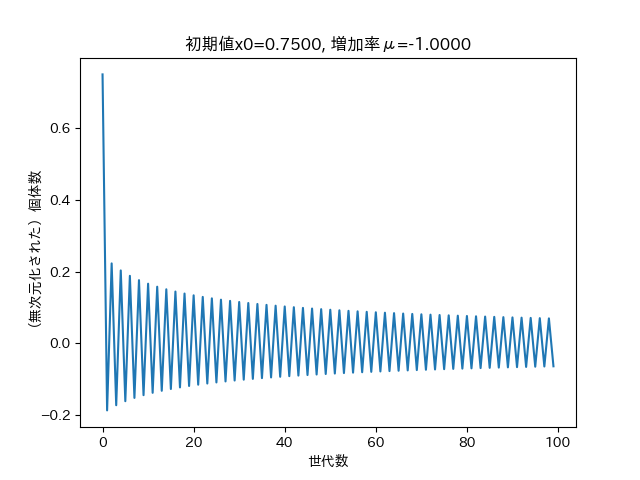
\includegraphics[width=70mm]
        {x0_0.7500-mu_-1.0000.png}
        \caption{初期値$x_0=0.75$,増加率$\mu=-1$}
        \label{fig:0.7500_-1.0000}
    \end{minipage}
    \begin{minipage}{0.50\hsize}
      \centering
      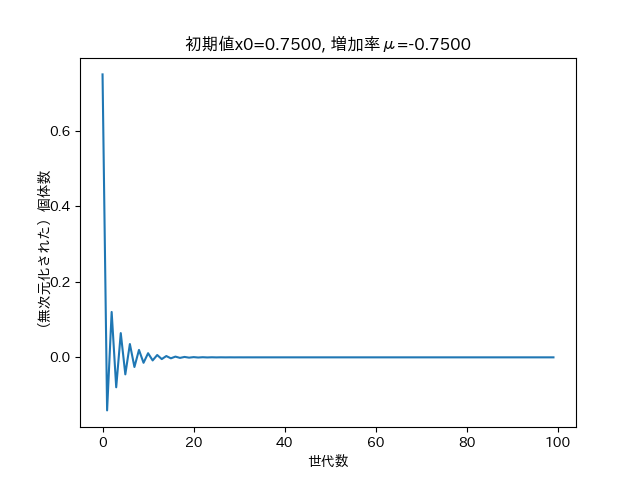
\includegraphics[width=70mm]
        {x0_0.7500-mu_-0.7500.png}
        \caption{初期値$x_0=0.75$,増加率$\mu=-0.75$}
        \label{fig:0.7500_-0.7500}
    \end{minipage}
  \end{tabular}
\end{figure}
\begin{figure}[htpb]
  \begin{tabular}{c}
    \begin{minipage}{0.50\hsize}
      \centering
      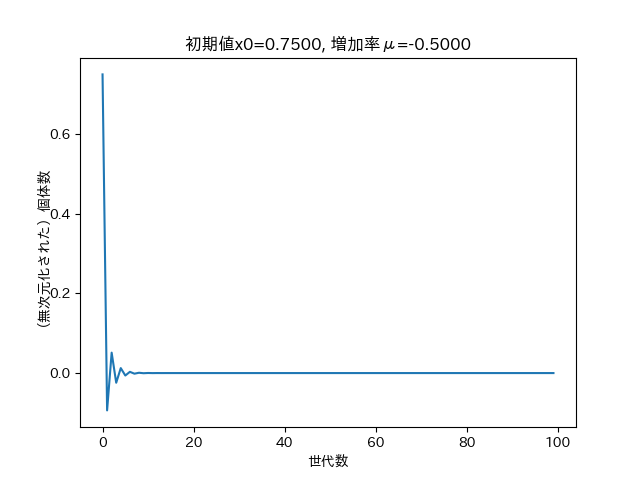
\includegraphics[width=70mm]
        {x0_0.7500-mu_-0.5000.png}
        \caption{初期値$x_0=0.75$,増加率$\mu=-0.5$}
        \label{fig:0.7500_-0.5000}
    \end{minipage}
    \begin{minipage}{0.50\hsize}
      \centering
      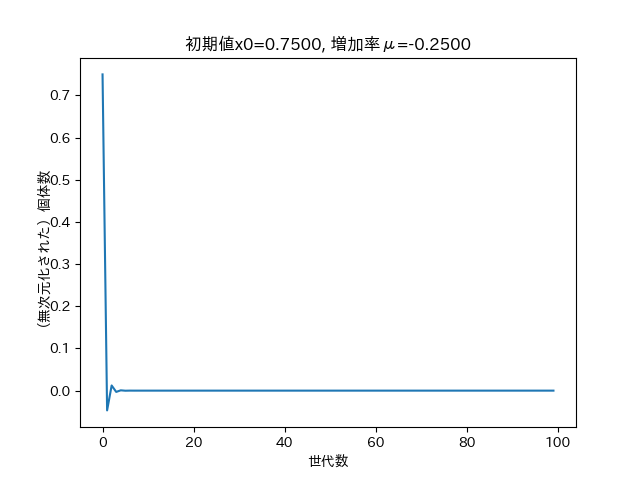
\includegraphics[width=70mm]
        {x0_0.7500-mu_-0.2500.png}
        \caption{初期値$x_0=0.75$,増加率$\mu=-0.25$}
        \label{fig:0.7500_-0.2500}
    \end{minipage}
  \end{tabular}
\end{figure}
\begin{figure}[htpb]
  \begin{tabular}{c}
    \begin{minipage}{0.50\hsize}
      \centering
      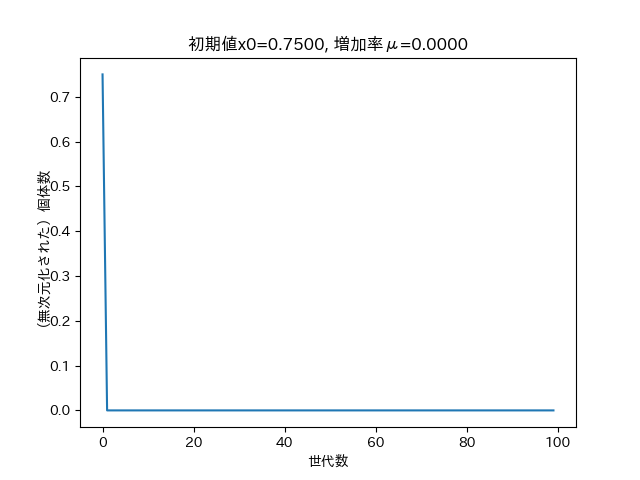
\includegraphics[width=70mm]
        {x0_0.7500-mu_0.0000.png}
        \caption{初期値$x_0=0.75$,増加率$\mu=0$}
        \label{fig:0.7500_0.0000}
    \end{minipage}
    \begin{minipage}{0.50\hsize}
      \centering
    \end{minipage}
  \end{tabular}
\end{figure}

\newpage
課題14.3-4: $\mu \ge 0$のときの個体数の変化.
\begin{figure}[htpb]
  \begin{tabular}{c}
    \begin{minipage}{0.50\hsize}
      \centering
      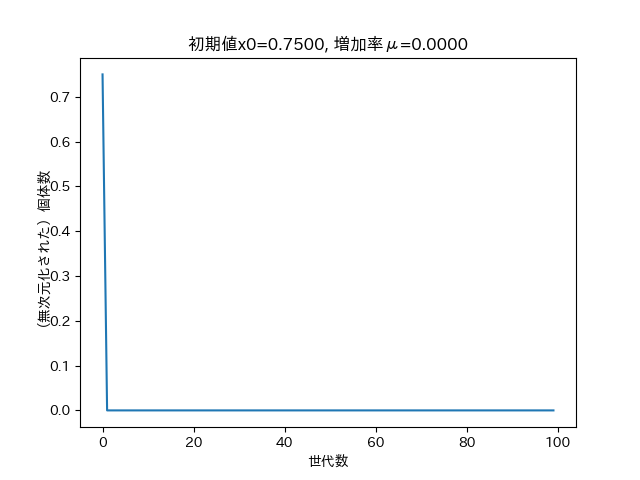
\includegraphics[width=70mm]
        {x0_0.7500-mu_0.0000.png}
        \caption{初期値$x_0=0.75$,増加率$\mu=0$}
        \label{fig:0.7500_0.0000}
    \end{minipage}
    \begin{minipage}{0.50\hsize}
      \centering
      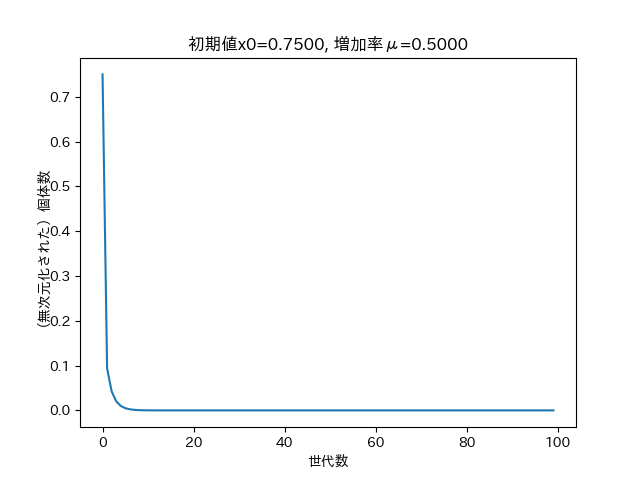
\includegraphics[width=70mm]
        {x0_0.7500-mu_0.5000.png}
        \caption{初期値$x_0=0.75$,増加率$\mu=0.5$}
        \label{fig:0.7500_0.5000}
    \end{minipage}
  \end{tabular}
\end{figure}
\begin{figure}[htpb]
  \begin{tabular}{c}
    \begin{minipage}{0.50\hsize}
      \centering
      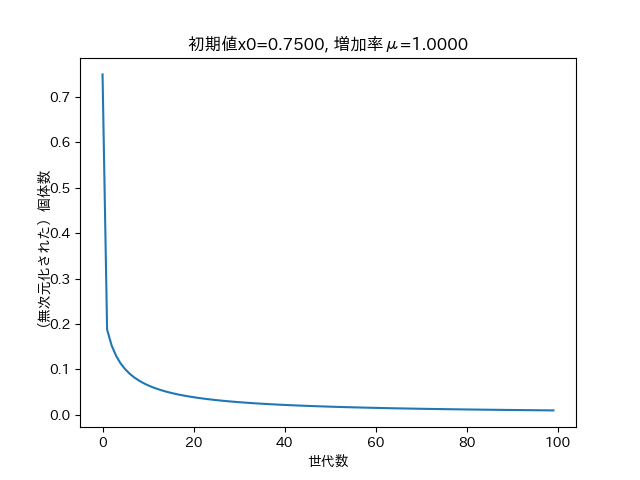
\includegraphics[width=70mm]
        {x0_0.7500-mu_1.0000.png}
        \caption{初期値$x_0=0.75$,増加率$\mu=1$}
        \label{fig:0.7500_1.0000}
    \end{minipage}
    \begin{minipage}{0.50\hsize}
      \centering
      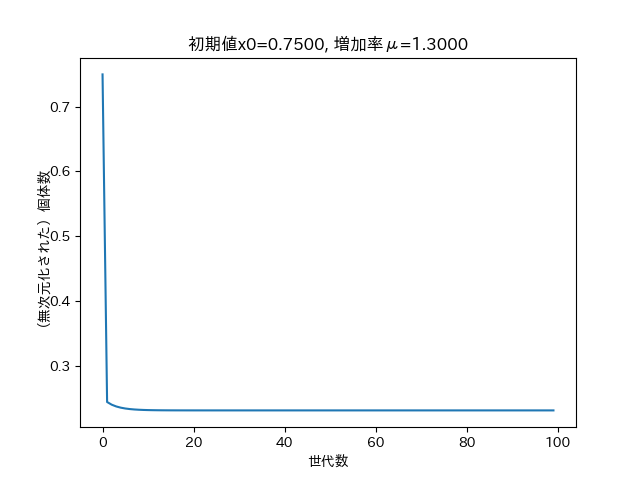
\includegraphics[width=70mm]
        {x0_0.7500-mu_1.3000.png}
        \caption{初期値$x_0=0.75$,増加率$\mu=1.3$}
        \label{fig:0.7500_1.3000}
    \end{minipage}
  \end{tabular}
\end{figure}
\begin{figure}[htpb]
  \begin{tabular}{c}
    \begin{minipage}{0.50\hsize}
      \centering
      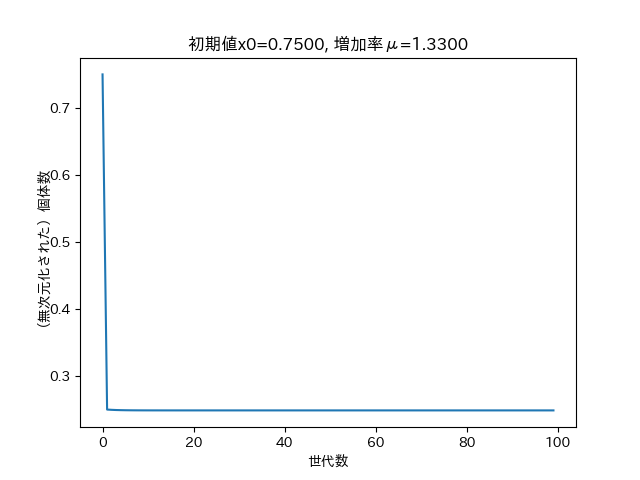
\includegraphics[width=70mm]
        {x0_0.7500-mu_1.3300.png}
        \caption{初期値$x_0=0.75$,増加率$\mu=1.33$}
        \label{fig:0.7500_1.3300}
    \end{minipage}
    \begin{minipage}{0.50\hsize}
      \centering
      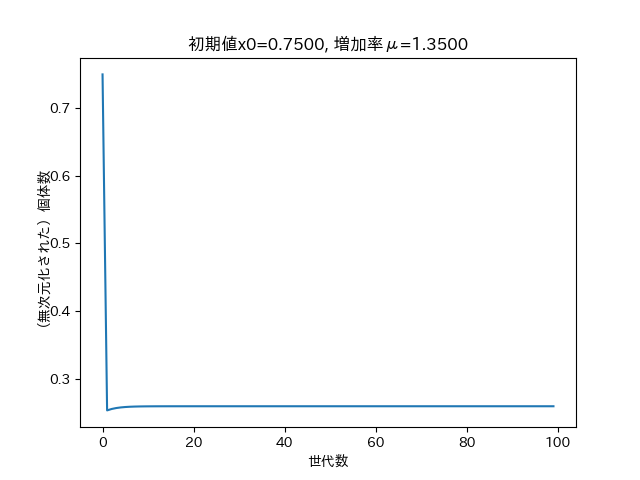
\includegraphics[width=70mm]
        {x0_0.7500-mu_1.3500.png}
        \caption{初期値$x_0=0.75$,増加率$\mu=1.35$}
        \label{fig:0.7500_1.3500}
    \end{minipage}
  \end{tabular}
\end{figure}
\begin{figure}[htpb]
  \begin{tabular}{c}
    \begin{minipage}{0.50\hsize}
      \centering
      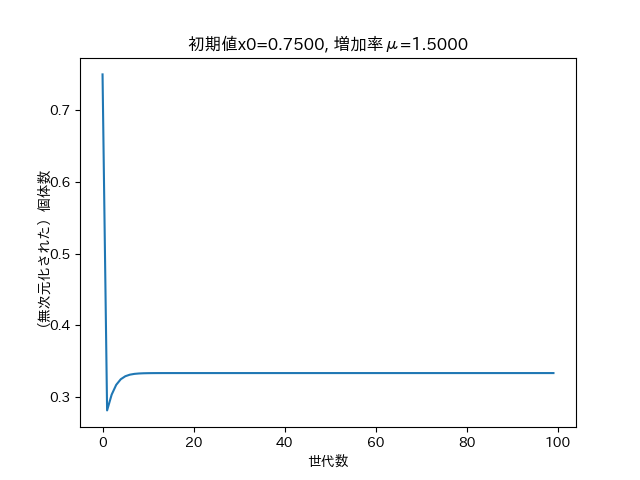
\includegraphics[width=70mm]
        {x0_0.7500-mu_1.5000.png}
        \caption{初期値$x_0=0.75$,増加率$\mu=1.5$}
        \label{fig:0.7500_1.5000}
    \end{minipage}
    \begin{minipage}{0.50\hsize}
      \centering
      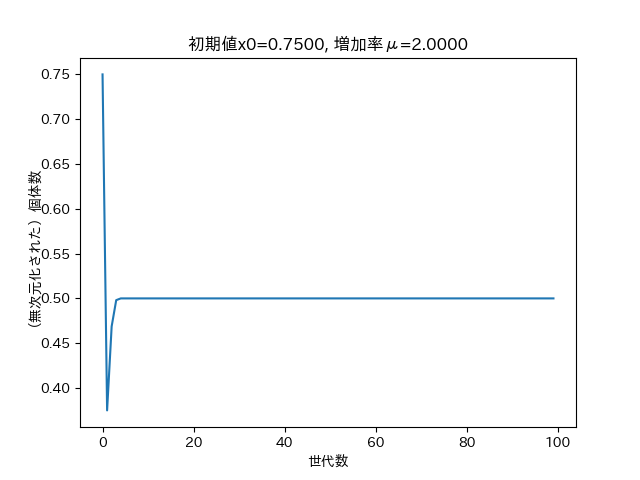
\includegraphics[width=70mm]
        {x0_0.7500-mu_2.0000.png}
        \caption{初期値$x_0=0.75$,増加率$\mu=2$}
        \label{fig:0.7500_2.0000}
    \end{minipage}
  \end{tabular}
\end{figure}
\begin{figure}[htpb]
  \begin{tabular}{c}
    \begin{minipage}{0.50\hsize}
      \centering
      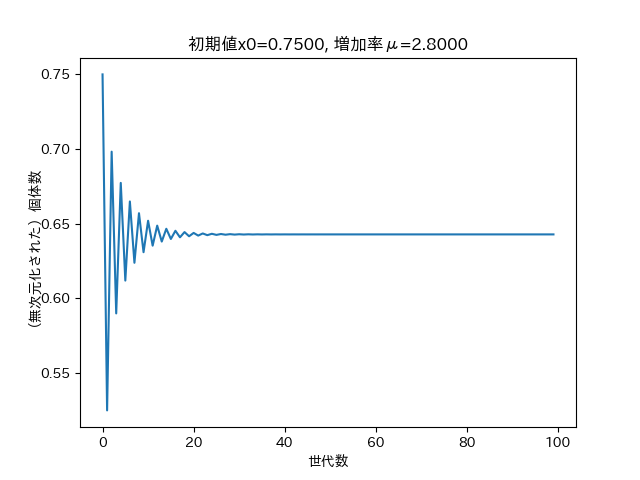
\includegraphics[width=70mm]
        {x0_0.7500-mu_2.8000.png}
        \caption{初期値$x_0=0.75$,増加率$\mu=2.8$}
        \label{fig:0.750_2.800}
    \end{minipage}
    \begin{minipage}{0.50\hsize}
      \centering
      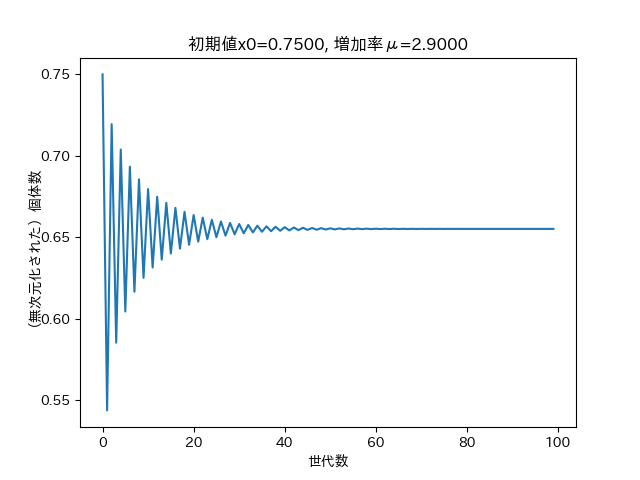
\includegraphics[width=70mm]
        {x0_0.7500-mu_2.9000.png}
        \caption{初期値$x_0=0.75$,増加率$\mu=2.9$}
        \label{fig:0.750_2.900}
    \end{minipage}
  \end{tabular}
\end{figure}
\begin{figure}[htpb]
  \begin{tabular}{c}
    \begin{minipage}{0.50\hsize}
      \centering
      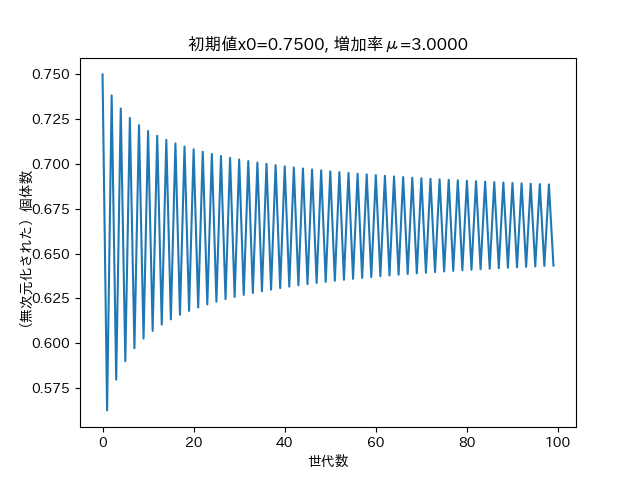
\includegraphics[width=70mm]
        {x0_0.7500-mu_3.0000.png}
        \caption{初期値$x_0=0.75$,増加率$\mu=3$}
        \label{fig:0.750_3.000}
    \end{minipage}
    \begin{minipage}{0.50\hsize}
      \centering
      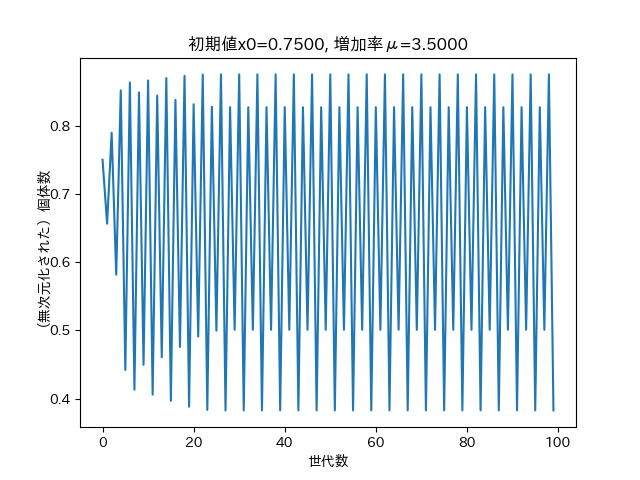
\includegraphics[width=70mm]
        {x0_0.7500-mu_3.5000.png}
        \caption{初期値$x_0=0.75$,増加率$\mu=3.5$}
        \label{fig:0.750_3.500}
    \end{minipage}
  \end{tabular}
\end{figure}
\begin{figure}[htpb]
  \begin{tabular}{c}
    \begin{minipage}{0.50\hsize}
      \centering
      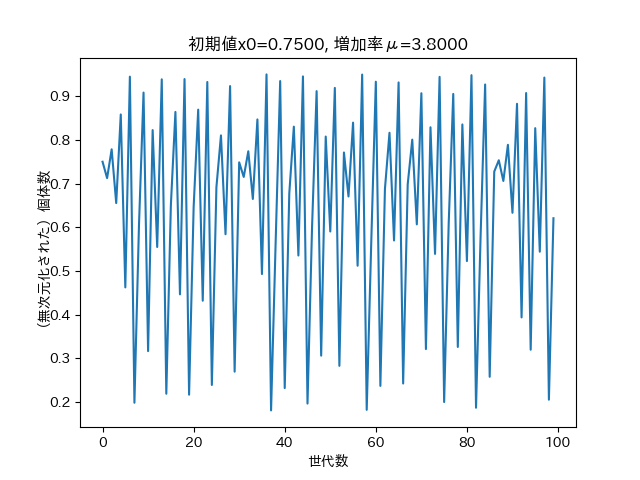
\includegraphics[width=70mm]
        {x0_0.7500-mu_3.8000.png}
        \caption{初期値$x_0=0.75$,増加率$\mu=3.8$}
        \label{fig:0.7500_3.8000}
    \end{minipage}
    \begin{minipage}{0.50\hsize}
      \centering
      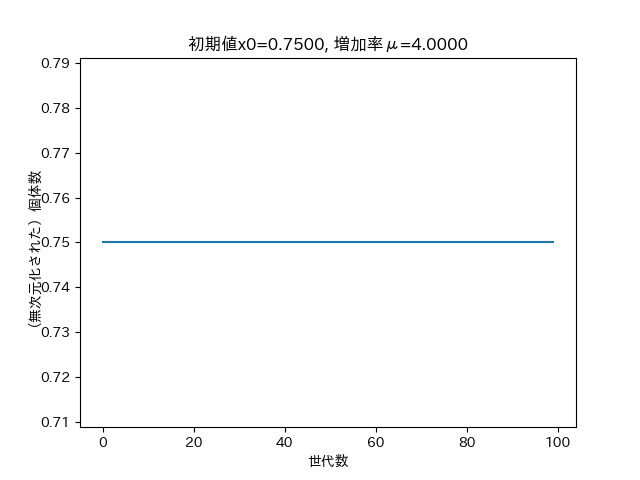
\includegraphics[width=70mm]
        {x0_0.7500-mu_4.0000.png}
        \caption{初期値$x_0=0.75$,増加率$\mu=4$}
        \label{fig:0.7500_4.0000}
    \end{minipage}
  \end{tabular}
\end{figure}
\begin{figure}[htpb]
  \begin{tabular}{c}
    \begin{minipage}{0.50\hsize}
      \centering
      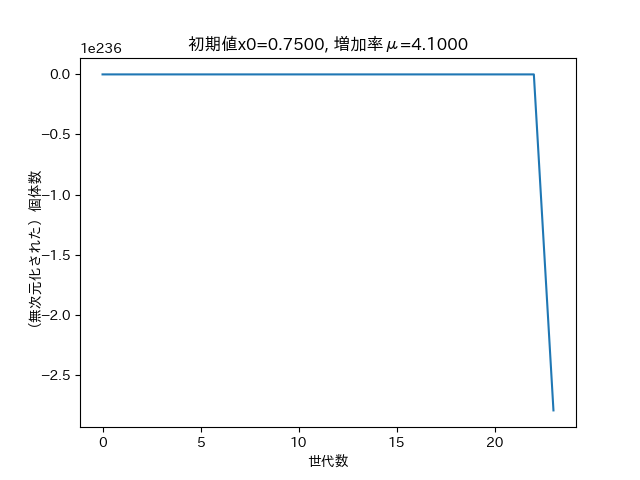
\includegraphics[width=70mm]
        {x0_0.7500-mu_4.1000.png}
        \caption{初期値$x_0=0.75$,増加率$\mu=4.1$}
        \label{fig:0.7500_3.8000}
    \end{minipage}
  \end{tabular}
\end{figure}

\newpage
\subsection{増加率を固定して初期値を変化させる}

課題14.3-6: 増加率$\mu$を一定として初期値$x_0$を変化させる.

$\mu=1$で固定した場合
\begin{figure}[htpb]
  \begin{tabular}{c}
    \begin{minipage}{0.50\hsize}
      \centering
      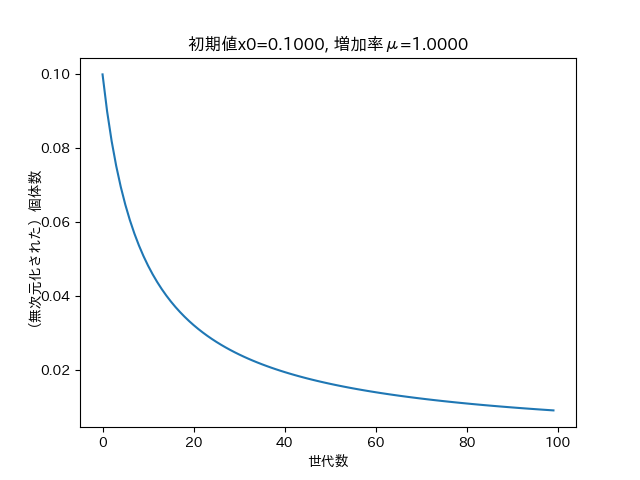
\includegraphics[width=70mm]
        {x0_0.1000-mu_1.0000.png}
        \caption{初期値$x_0=0.1$,増加率$\mu=1$}
        \label{fig:0.1000_1.0000}
    \end{minipage}
    \begin{minipage}{0.50\hsize}
      \centering
      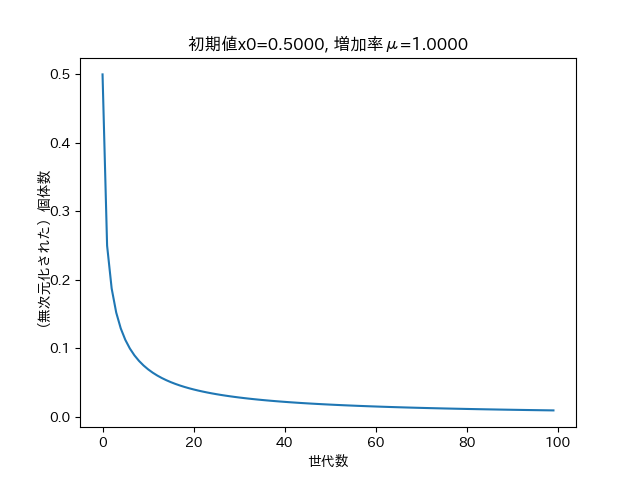
\includegraphics[width=70mm]
        {x0_0.5000-mu_1.0000.png}
        \caption{初期値$x_0=0.5$,増加率$\mu=1$}
        \label{fig:0.5000_1.0000}
    \end{minipage}
  \end{tabular}
\end{figure}
\begin{figure}[htpb]
  \begin{tabular}{c}
    \begin{minipage}{0.50\hsize}
      \centering
      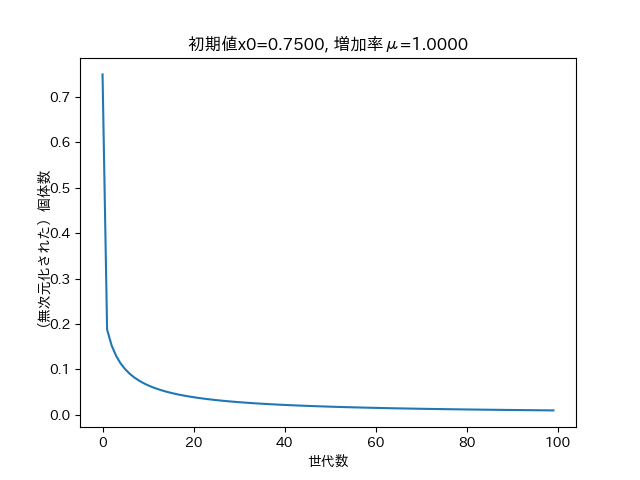
\includegraphics[width=70mm]
        {x0_0.7500-mu_1.0000.png}
        \caption{初期値$x_0=0.75$,増加率$\mu=1$}
        \label{fig:0.7500_1.0000-2}
    \end{minipage}
    \begin{minipage}{0.50\hsize}
      \centering
      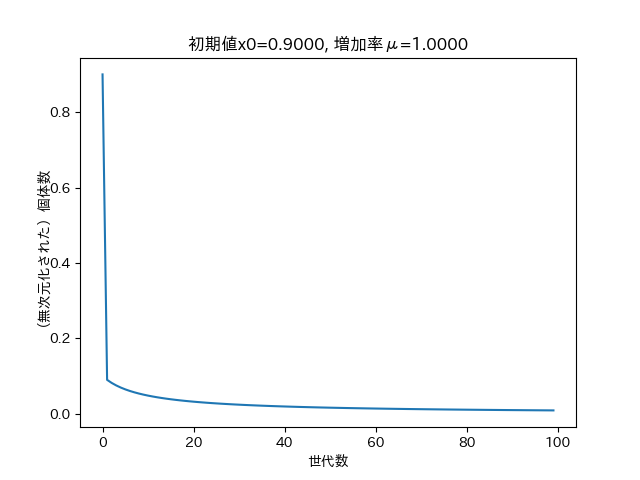
\includegraphics[width=70mm]
        {x0_0.9000-mu_1.0000.png}
        \caption{初期値$x_0=0.9$,増加率$\mu=1$}
        \label{fig:0.9000_1.0000}
    \end{minipage}
  \end{tabular}
\end{figure}

\newpage
$\mu=2.9$で固定した場合

$x_* \ne 0$を不動点とするとき,
\begin{equation}
  x_* = \mu x_* (1-x_*)
\end{equation}
より
\begin{equation}
  x_* = 1 - \frac{1}{\mu}.
\end{equation}
$\mu=2.9$とすると$x_*=0.65517\ldots$.
\begin{figure}[htpb]
  \begin{tabular}{c}
    \begin{minipage}{0.50\hsize}
      \centering
      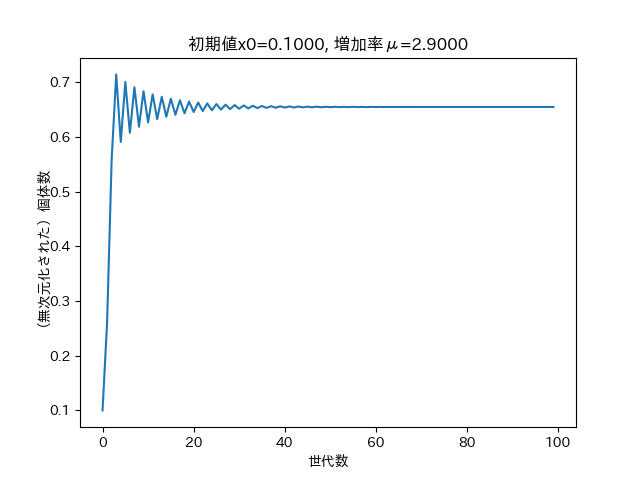
\includegraphics[width=70mm]
        {x0_0.1000-mu_2.9000.png}
        \caption{初期値$x_0=0.1$,増加率$\mu=2.9$}
        \label{fig:0.1000_2.9000}
    \end{minipage}
    \begin{minipage}{0.50\hsize}
      \centering
      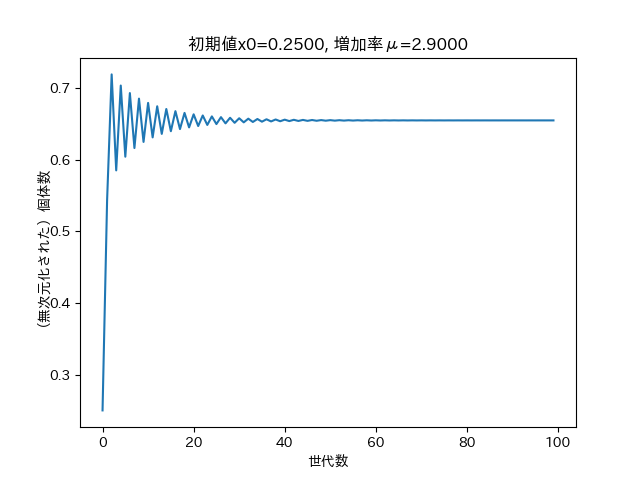
\includegraphics[width=70mm]
        {x0_0.2500-mu_2.9000.png}
        \caption{初期値$x_0=0.25$,増加率$\mu=2.9$}
        \label{fig:0.2500_2.9000}
    \end{minipage}
  \end{tabular}
\end{figure}
\begin{figure}[htpb]
  \begin{tabular}{c}
    \begin{minipage}{0.50\hsize}
      \centering
      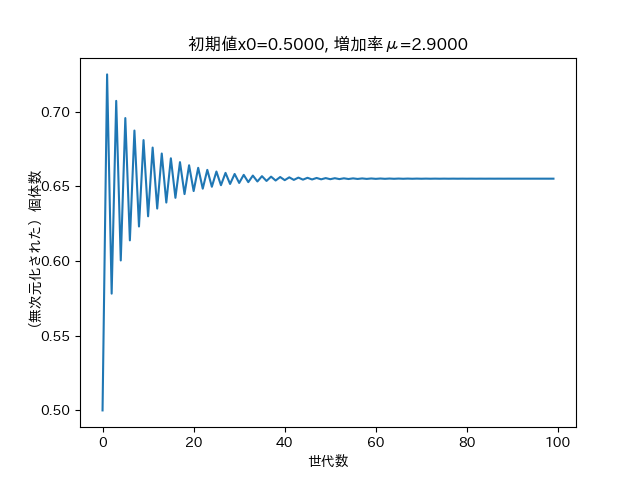
\includegraphics[width=70mm]
        {x0_0.5000-mu_2.9000.png}
        \caption{初期値$x_0=0.5$,増加率$\mu=2.9$}
        \label{fig:0.5000_2.9000}
    \end{minipage}
    \begin{minipage}{0.50\hsize}
      \centering
      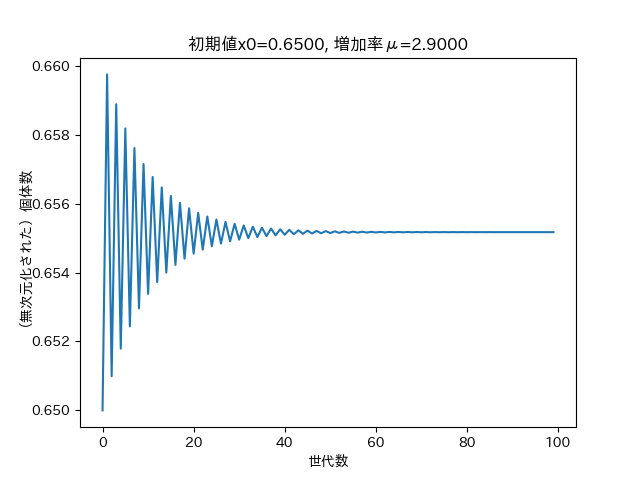
\includegraphics[width=70mm]
        {x0_0.6500-mu_2.9000.png}
        \caption{初期値$x_0=0.65$,増加率$\mu=2.9$}
        \label{fig:0.6500_2.9000}
    \end{minipage}
  \end{tabular}
\end{figure}
\begin{figure}[htpb]
  \begin{tabular}{c}
    \begin{minipage}{0.50\hsize}
      \centering
      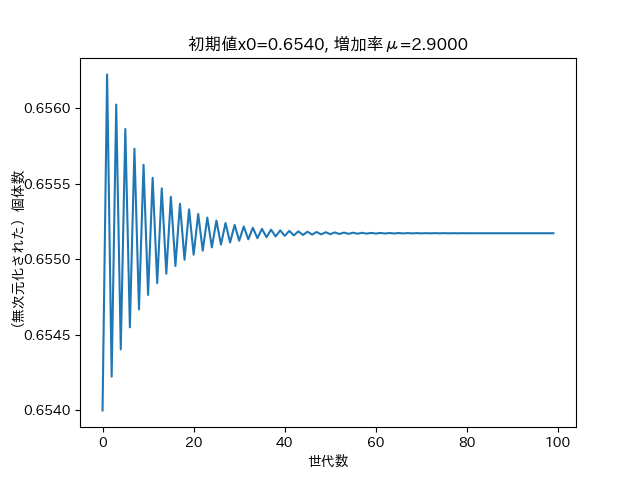
\includegraphics[width=70mm]
        {x0_0.6540-mu_2.9000.png}
        \caption{初期値$x_0=0.654$,増加率$\mu=2.9$}
        \label{fig:0.6540_2.9000}
    \end{minipage}
    \begin{minipage}{0.50\hsize}
      \centering
      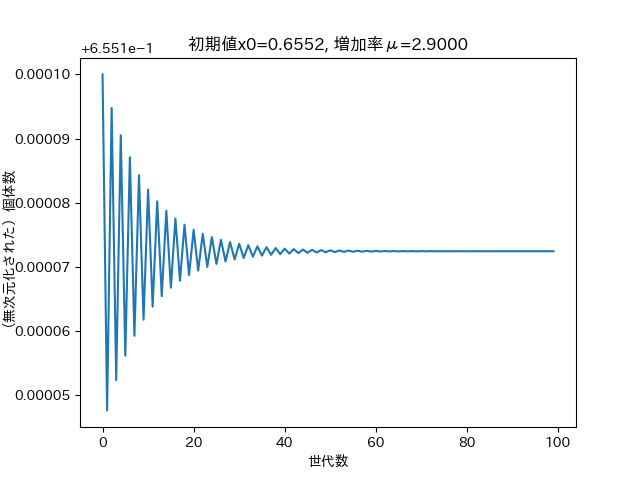
\includegraphics[width=70mm]
        {x0_0.6552-mu_2.9000.png}
        \caption{初期値$x_0=0.6552$,増加率$\mu=2.9$}
        \label{fig:0.6552_2.9000}
    \end{minipage}
  \end{tabular}
\end{figure}
\begin{figure}[htpb]
  \begin{tabular}{c}
    \begin{minipage}{0.50\hsize}
      \centering
      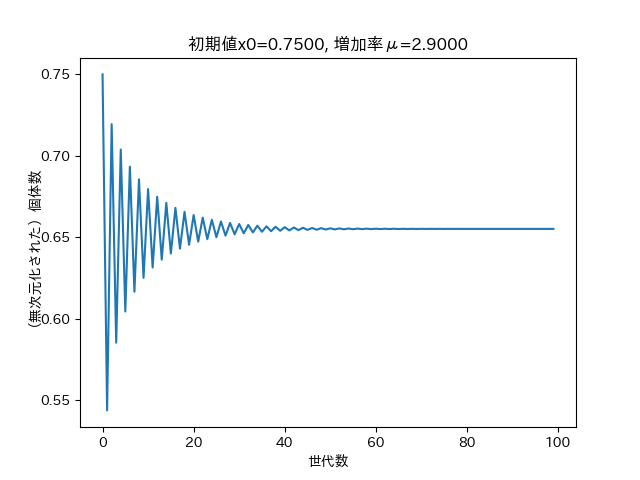
\includegraphics[width=70mm]
        {x0_0.7500-mu_2.9000.png}
        \caption{初期値$x_0=0.75$,増加率$\mu=2.9$}
        \label{fig:0.7500_2.9000-2}
    \end{minipage}
    \begin{minipage}{0.50\hsize}
      \centering
      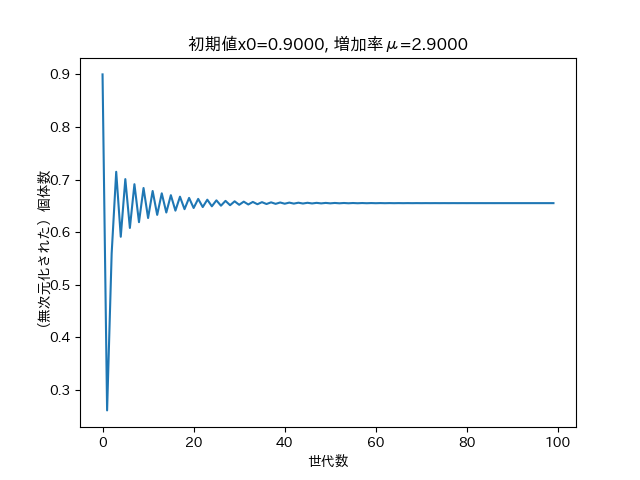
\includegraphics[width=70mm]
        {x0_0.9000-mu_2.9000.png}
        \caption{初期値$x_0=0.9$,増加率$\mu=2.9$}
        \label{fig:0.9000_2.9000}
    \end{minipage}
  \end{tabular}
\end{figure}

\newpage
$\mu=3.3$で固定した場合
\begin{figure}[htpb]
  \begin{tabular}{c}
    \begin{minipage}{0.50\hsize}
      \centering
      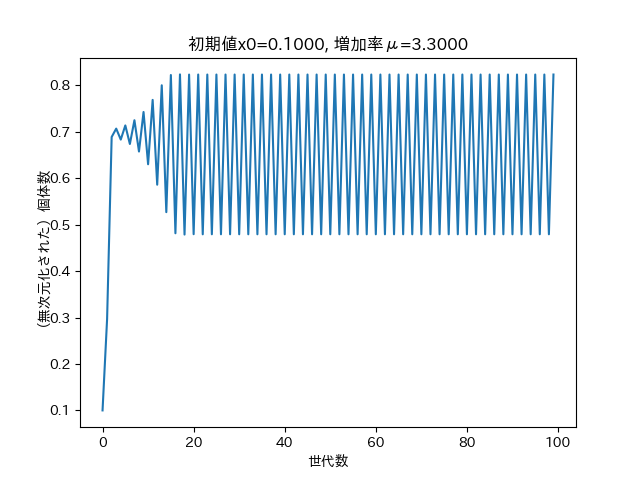
\includegraphics[width=70mm]
        {x0_0.1000-mu_3.3000.png}
        \caption{初期値$x_0=0.1$,増加率$\mu=3.3$}
        \label{fig:0.1000_3.3000}
    \end{minipage}
    \begin{minipage}{0.50\hsize}
      \centering
      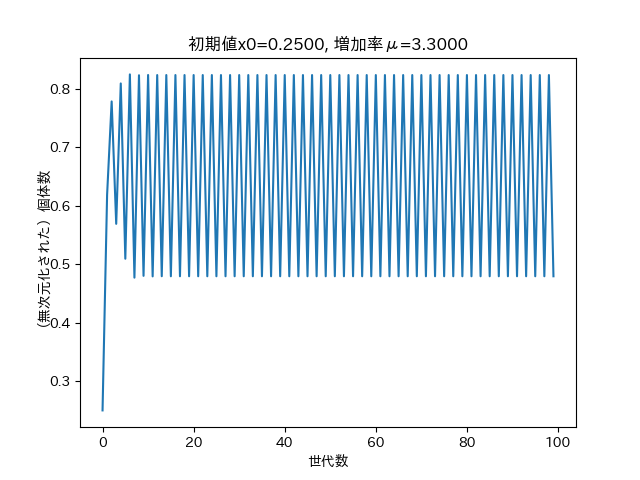
\includegraphics[width=70mm]
        {x0_0.2500-mu_3.3000.png}
        \caption{初期値$x_0=0.25$,増加率$\mu=3.3$}
        \label{fig:0.2500_3.3000}
    \end{minipage}
  \end{tabular}
\end{figure}
\begin{figure}[htpb]
  \begin{tabular}{c}
    \begin{minipage}{0.50\hsize}
      \centering
      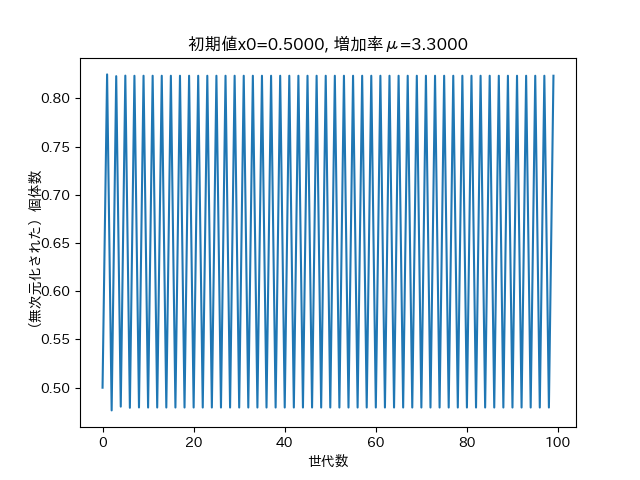
\includegraphics[width=70mm]
        {x0_0.5000-mu_3.3000.png}
        \caption{初期値$x_0=0.5$,増加率$\mu=3.3$}
        \label{fig:0.5000_3.3000}
    \end{minipage}
    \begin{minipage}{0.50\hsize}
      \centering
      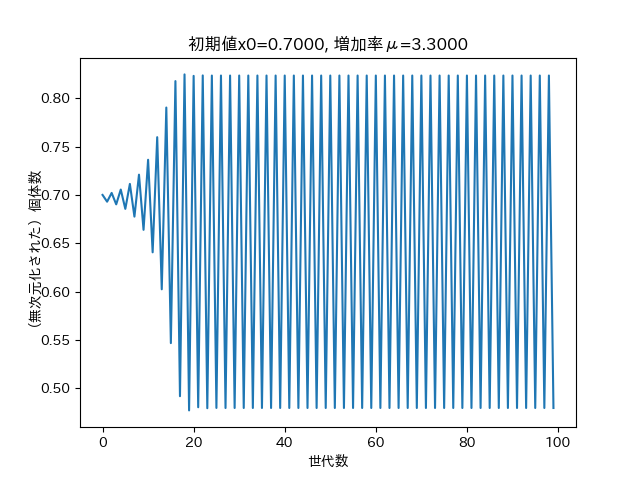
\includegraphics[width=70mm]
        {x0_0.7000-mu_3.3000.png}
        \caption{初期値$x_0=0.7$,増加率$\mu=3.3$}
        \label{fig:0.7000_3.3000}
    \end{minipage}
  \end{tabular}
\end{figure}
\begin{figure}[htpb]
  \begin{tabular}{c}
    \begin{minipage}{0.50\hsize}
      \centering
      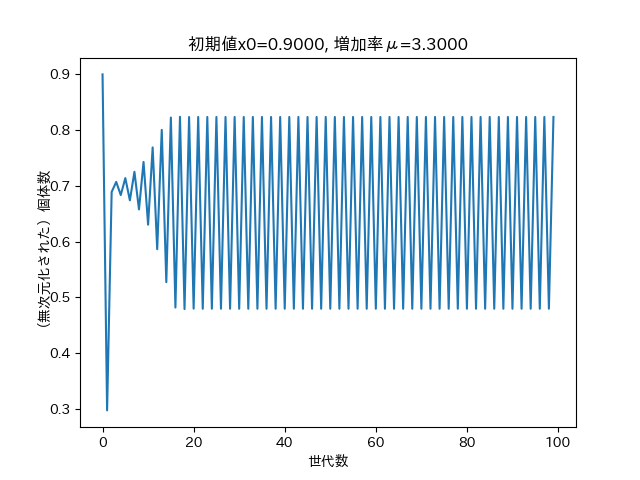
\includegraphics[width=70mm]
        {x0_0.9000-mu_3.3000.png}
        \caption{初期値$x_0=0.9$,増加率$\mu=3.3$}
        \label{fig:0.9000_3.3000}
    \end{minipage}
  \end{tabular}
\end{figure}

\newpage
$\mu=3.5$で固定した場合
\begin{figure}[htpb]
  \begin{tabular}{c}
    \begin{minipage}{0.50\hsize}
      \centering
      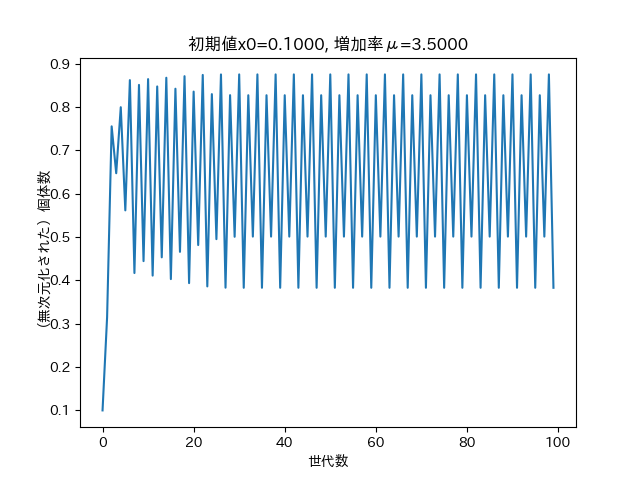
\includegraphics[width=70mm]
        {x0_0.1000-mu_3.5000.png}
        \caption{初期値$x_0=0.1$,増加率$\mu=3.5$}
        \label{fig:0.1000_3.5000}
    \end{minipage}
    \begin{minipage}{0.50\hsize}
      \centering
      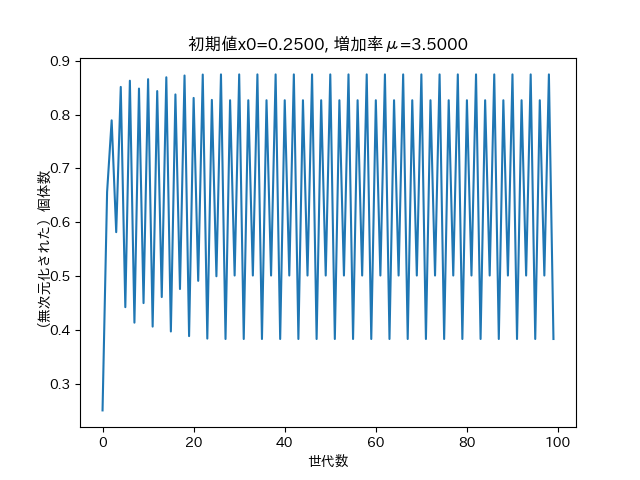
\includegraphics[width=70mm]
        {x0_0.2500-mu_3.5000.png}
        \caption{初期値$x_0=0.25$,増加率$\mu=3.5$}
        \label{fig:0.2500_3.5000}
    \end{minipage}
  \end{tabular}
\end{figure}
\begin{figure}[htpb]
  \begin{tabular}{c}
    \begin{minipage}{0.50\hsize}
      \centering
      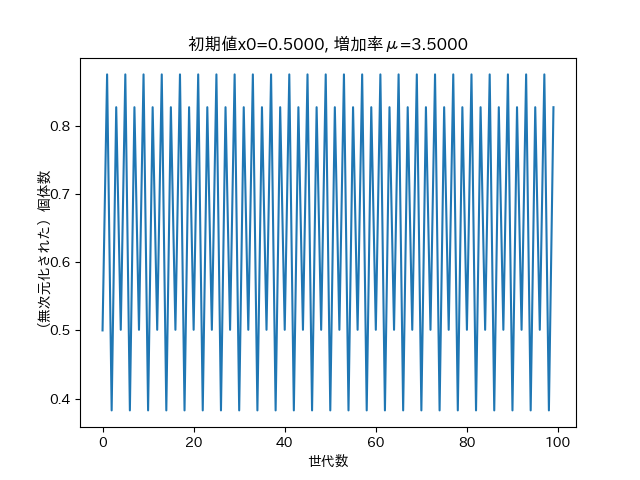
\includegraphics[width=70mm]
        {x0_0.5000-mu_3.5000.png}
        \caption{初期値$x_0=0.5$,増加率$\mu=3.5$}
        \label{fig:0.5000_3.5000}
    \end{minipage}
    \begin{minipage}{0.50\hsize}
      \centering
      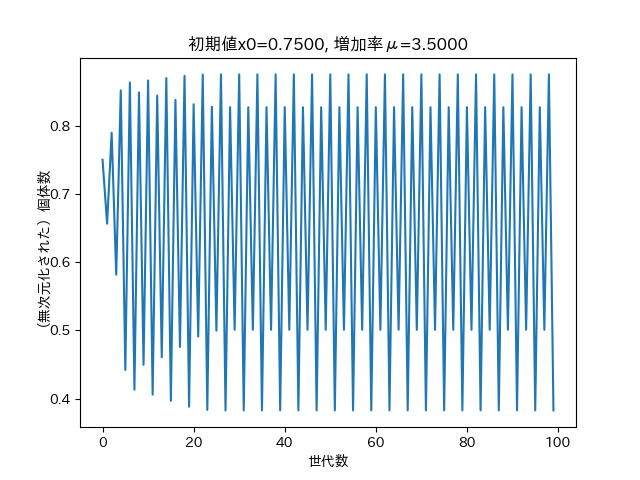
\includegraphics[width=70mm]
        {x0_0.7500-mu_3.5000.png}
        \caption{初期値$x_0=0.75$,増加率$\mu=3.5$}
        \label{fig:0.7500_3.5000-2}
    \end{minipage}
  \end{tabular}
\end{figure}
\begin{figure}[htpb]
  \begin{tabular}{c}
    \begin{minipage}{0.50\hsize}
      \centering
      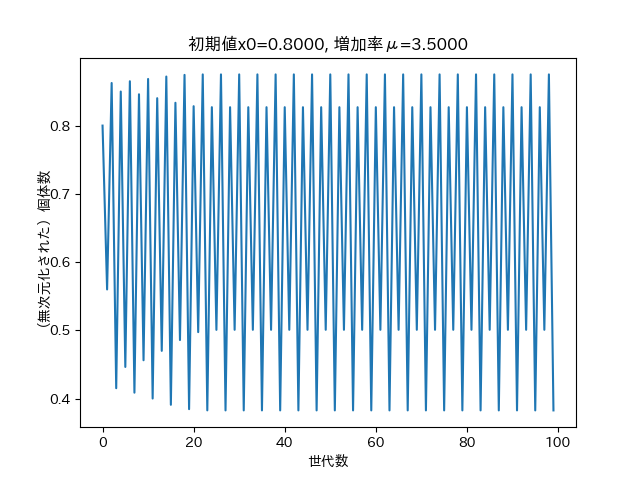
\includegraphics[width=70mm]
        {x0_0.8000-mu_3.5000.png}
        \caption{初期値$x_0=0.8$,増加率$\mu=3.5$}
        \label{fig:0.8000_3.5000}
    \end{minipage}
    \begin{minipage}{0.50\hsize}
      \centering
      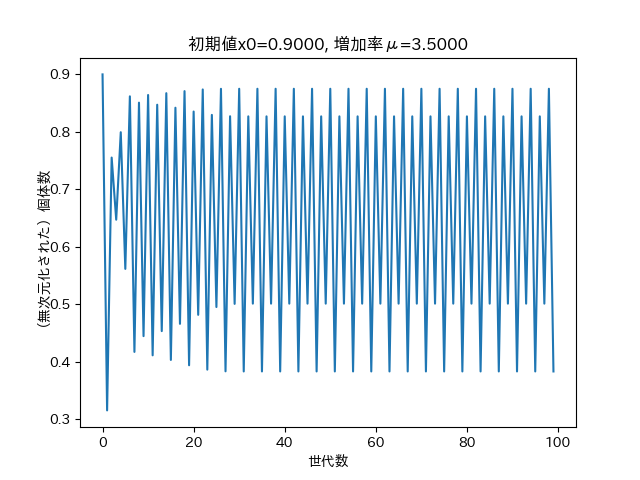
\includegraphics[width=70mm]
        {x0_0.9000-mu_3.5000.png}
        \caption{初期値$x_0=0.9$,増加率$\mu=3.5$}
        \label{fig:0.9000_3.5000}
    \end{minipage}
  \end{tabular}
\end{figure}

\newpage
$\mu=3.8$で固定した場合
\begin{figure}[htpb]
  \begin{tabular}{c}
    \begin{minipage}{0.50\hsize}
      \centering
      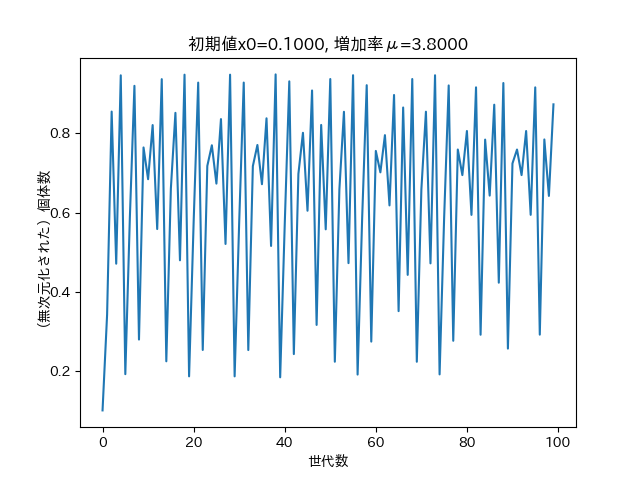
\includegraphics[width=70mm]
        {x0_0.1000-mu_3.8000.png}
        \caption{初期値$x_0=0.1$,増加率$\mu=3.8$}
        \label{fig:0.1000_3.8000}
    \end{minipage}
    \begin{minipage}{0.50\hsize}
      \centering
      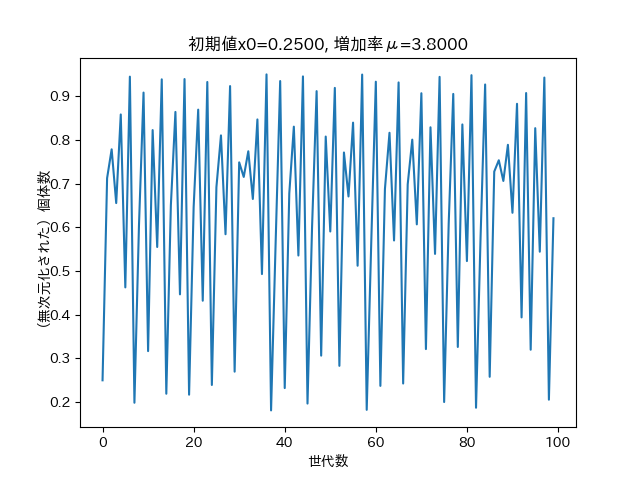
\includegraphics[width=70mm]
        {x0_0.2500-mu_3.8000.png}
        \caption{初期値$x_0=0.25$,増加率$\mu=3.8$}
        \label{fig:0.2500_3.8000}
    \end{minipage}
  \end{tabular}
\end{figure}
\begin{figure}[htpb]
  \begin{tabular}{c}
    \begin{minipage}{0.50\hsize}
      \centering
      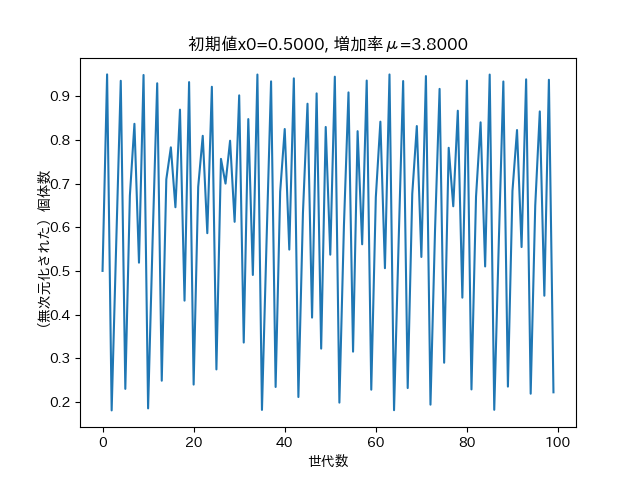
\includegraphics[width=70mm]
        {x0_0.5000-mu_3.8000.png}
        \caption{初期値$x_0=0.5$,増加率$\mu=3.8$}
        \label{fig:0.5000_3.8000}
    \end{minipage}
    \begin{minipage}{0.50\hsize}
      \centering
      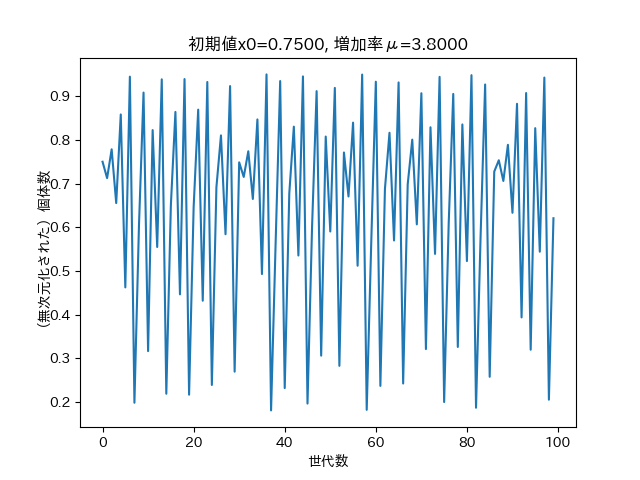
\includegraphics[width=70mm]
        {x0_0.7500-mu_3.8000.png}
        \caption{初期値$x_0=0.75$,増加率$\mu=3.8$}
        \label{fig:0.7500_3.8000-2}
    \end{minipage}
  \end{tabular}
\end{figure}
\begin{figure}[htpb]
  \begin{tabular}{c}
    \begin{minipage}{0.50\hsize}
      \centering
      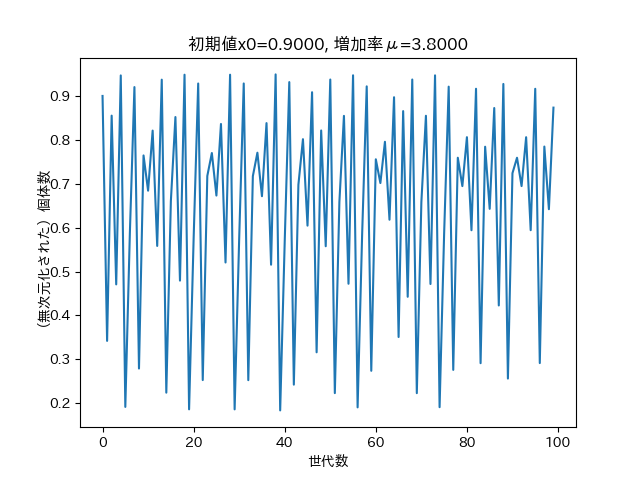
\includegraphics[width=70mm]
        {x0_0.9000-mu_3.8000.png}
        \caption{初期値$x_0=0.9$,増加率$\mu=3.8$}
        \label{fig:0.9000_3.8000}
    \end{minipage}
  \end{tabular}
\end{figure}

\subsection{ファイゲンバウムによる観察の確認}

ここでは初期値を$x_0=0.75$に固定する.
\begin{figure}[htpb]
  \begin{tabular}{c}
    \begin{minipage}{0.50\hsize}
      \centering
      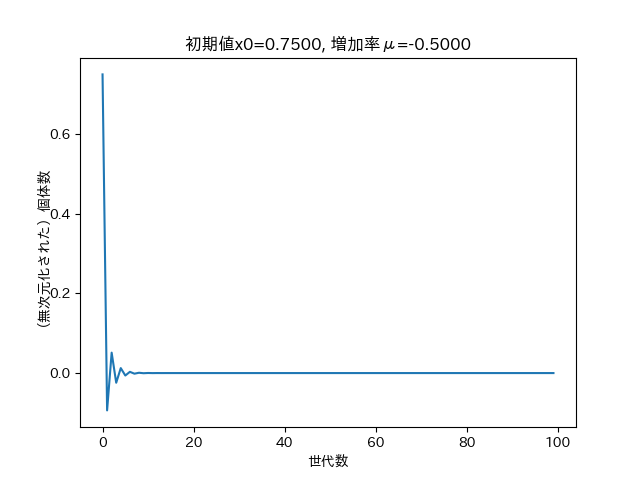
\includegraphics[width=70mm]
        {x0_0.7500-mu_-0.5000.png}
        \caption{増加率$\mu=-0.5$のとき個体数は定常解のゼロに漸近し,時間が経つとゼロで安定する}
        \label{fig:0.7500_-0.5000-2}
    \end{minipage}
    \begin{minipage}{0.50\hsize}
      \centering
      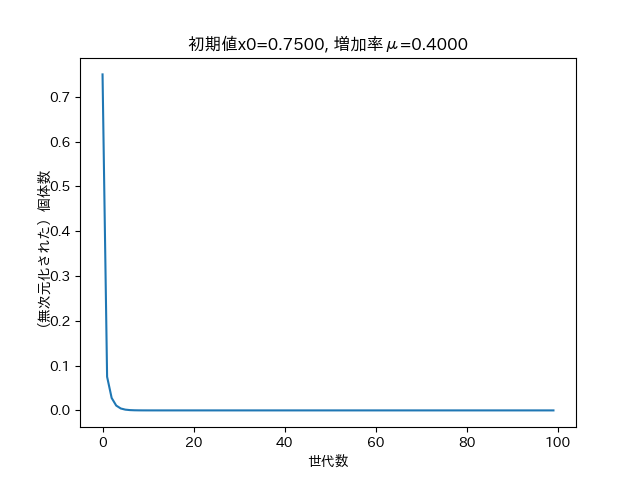
\includegraphics[width=70mm]
        {x0_0.7500-mu_0.4000.png}
        \caption{増加率$\mu=0.4$のとき個体数は定常解のゼロに漸近し,時間が経つとゼロで安定する}
        \label{fig:0.7500_0.4000}
    \end{minipage}
  \end{tabular}
\end{figure}
\begin{figure}
  \begin{tabular}{c}
    \begin{minipage}{0.50\hsize}
      \centering
      \includegraphics[width=70mm]
        {x0_0.7500-mu_1.5000.png}
        \caption{増加率$\mu=1.5$のとき個体数は非自明な定常解に漸近し,時間が経つとその定常解で安定する}
        \label{fig:0.7500_1.5000-2}
    \end{minipage}
    \begin{minipage}{0.50\hsize}
      \centering
      \includegraphics[width=70mm]
        {x0_0.7500-mu_2.4000.png}
        \caption{増加率$\mu=2.4$のとき個体数は非自明な定常解に振動しながら漸近し,時間が経つとその定常解で安定する}
        \label{fig:0.7500_2.4000}
    \end{minipage}    
  \end{tabular}
\end{figure}
\begin{figure}
  \begin{tabular}{c}
    \begin{minipage}{0.50\hsize}
      \centering
      \includegraphics[width=70mm]
        {x0_0.7500-mu_3.2000.png}
        \caption{増加率$\mu=3.2$のとき時間が経つと二重周期解に安定する}
        \label{fig:0.7500_3.2000}
    \end{minipage}
    \begin{minipage}{0.50\hsize}
      \centering
      \includegraphics[width=70mm]
        {x0_0.7500-mu_3.5000.png}
        \caption{増加率$\mu=3.5$のとき時間が経つと四重周期解に安定する}
        \label{fig:0.7500_3.5000-2}
    \end{minipage}    
  \end{tabular}
\end{figure}
\begin{figure}
  \begin{tabular}{c}
    \begin{minipage}{0.50\hsize}
      \centering
      \includegraphics[width=70mm]
        {x0_0.7500-mu_3.6000.png}
        \caption{増加率$\mu=3.6$のときカオス的な振る舞いをする}
        \label{fig:0.7500_3.6000}
    \end{minipage}
    \begin{minipage}{0.50\hsize}
      \centering
      \includegraphics[width=70mm]
        {x0_0.7500-mu_3.8264.png}
        \caption{増加率$\mu=3.8264$のとき安定に見える期間とそれが崩れたのち再び安定に見える状態となる間欠状態が見られる}
        \label{fig:0.7500_3.8264}
    \end{minipage}    
  \end{tabular}
\end{figure}
\begin{figure}
  \begin{tabular}{c}
    \begin{minipage}{0.50\hsize}
      \centering
      \includegraphics[width=70mm]
        {x0_0.7500-mu_3.8274.png}
        \caption{増加率$\mu=3.8274$のとき間欠状態が見られる}
        \label{fig:0.7500_3.8274}
    \end{minipage}
    \begin{minipage}{0.50\hsize}
      \centering
      \includegraphics[width=70mm]
        {x0_0.7500-mu_3.8284-N_300.png}
        \caption{増加率$\mu=3.8284$のとき間欠状態が見られる(但し試行回数を300回に増やす)}
        \label{fig:0.7500_3.8284}
    \end{minipage}    
  \end{tabular}
\end{figure}
\begin{figure}
  \begin{tabular}{c}
    \begin{minipage}{0.50\hsize}
      \centering
      \includegraphics[width=70mm]
        {x0_0.7500-mu_3.8304.png}
        \caption{増加率$\mu=3.8304$のとき二重周期解で安定となる}
        \label{fig:0.7500_3.8304}
    \end{minipage}
    \begin{minipage}{0.50\hsize}
      \centering
      \includegraphics[width=70mm]
        {x0_0.7500-mu_4.0000.png}
        \caption{増加率$\mu=4$のとき初期値$0.75$が安定である}
        \label{fig:0.7500_4.0000}
    \end{minipage}    
  \end{tabular}
\end{figure}

\newpage


\end{document}